\documentclass[10pt]{article}
\usepackage[margin=0.78in]{geometry}
\usepackage[T1]{fontenc}
\usepackage{lmodern}
\usepackage{microtype}
\usepackage{booktabs,tabularx,array}
\usepackage{graphicx}
\usepackage{hyperref}
\usepackage{xcolor}
\emergencystretch=3em
\hypersetup{colorlinks=true,linkcolor=blue!55!black,urlcolor=blue!55!black}
\title{IDM-Viz: Impact-Aware Drift Monitoring\\A Reproducible Phase 3 Implementation and Audit}
\author{Umar Behram (23I-2604) \and Ahmed Bilal (23I-2581)\\Department of AI and Data Science, FAST-NUCES Islamabad}
\date{Day 1 research-improvement edition -- 15 November 2026}
\begin{document}
\maketitle
\begin{abstract}
This report consolidates the controlled synthetic evidence and protocol audit for IDM-Viz, a monitoring prototype that coordinates input alarms, descriptive feature evidence, estimated accuracy, delayed-label verification, and a shared evidence view. The submitted Phase 2 DOCX remains the methodological basis. Phase 3 implements a frozen logistic study across seven conditions and adds separately identified XOR/tree and cumulative-label adaptation extensions. Existing receipts report complete reruns and exact artifact comparisons; the present session independently inspected source contracts and archive hashes but did not rerun the experiment suite. Results remain synthetic and do not establish real-world transfer, causal explanation, human benefit, or population safety.
\end{abstract}

\section{Basis and scope}
\begin{sloppypar}
The authoritative methodological source is the submitted Phase 2 methodology \cite{phase2methodology}, located at \path{docs/23i-2604_23i-2581DAV-phase2.docx}. Its SHA-256 is recorded in \path{HASHES.sha256}. The Phase 3 implementation plan narrows that basis to a reproducible controlled study. No instructor feedback was received. The original submitted Phase 3 archive remains unchanged and is separately hash identified in the accompanying preservation record. This package is subsequent research work, not a resubmission snapshot.
\end{sloppypar}

\begin{table}[h]
\small\centering
\begin{tabularx}{\linewidth}{p{.22\linewidth}XX}
\toprule
Phase 2 objective & Phase 3 implementation and located evidence & Limitations and deferred scope\\
\midrule
Detect distribution change & Original-feature two-sided KS tests with Holm correction; three frozen PCA coordinates provide additional evidence. Seven controlled conditions include stationary, mean, conditional, recurrent, and dependence changes. & Alarms concern input distributions, not predictive harm. Synthetic onset is known; no natural onset recall is established.\\
Explain drift & Feature rankings, clusters, and a coordinated feature view. & Evidence is descriptive, not causal attribution. Dependence changes need not alter univariate marginals.\\
Estimate impact & Frozen logistic classifier, separate correctness calibration, Average Confidence, and plug-in Poisson-binomial intervals. & Intervals omit calibration parameter uncertainty and have no arbitrary-shift guarantee. Observed coverage is below nominal.\\
Verify with labels & Prediction persistence precedes scheduled label release; source implements explicit phase ordering and as-of filtering. & Broker is an API boundary, not a security sandbox. Accuracy is retrospective until labels arrive.\\
Coordinate evidence & Shared batch axis joins alarms, feature distances, impact estimates, and release status. & A visualization has not been shown to improve analyst decisions.\\
Evaluate response & Separate exploratory cumulative-refit adaptation study on selected C3 and XOR X3. & Outcome-informed selection; only two synthetic changes and one adapter. Not general adaptation evidence.\\
\bottomrule
\end{tabularx}
\end{table}

\section{Methods and implementation}
For each of 30 final seeds, the original task uses disjoint samples of 4,000 training, 2,000 calibration, 2,000 historical-reference, and 12,000 monitoring observations per condition. Monitoring data are processed in 24 batches of 500. A frozen logistic regression (\texttt{C=1}, 500 iterations) is fitted after training-only standardization. Three-component PCA and three-cluster MiniBatchKMeans are also training-only. Isotonic correctness calibration is fitted on the separate calibration sample; predictions retain the original 0.5 class threshold.

Baseline inputs are generated from independent standard-normal innovations. The dependence condition changes correlation of $X_0,X_1$ from 0.3 to 0.9 while retaining unit marginals through $X_1=.9Z_0+\sqrt{1-.9^2}Z_1$. Source inspection confirms this current formula and the input-only FeatureBatch interface. The condition does not change the conditional label rule beyond its dependence-mediated input change. The other conditions introduce nuisance or predictive mean shifts, conditional probability reversal, gradual reversal, and recurrence.

At each batch, the runner persists predictions before releasing labels at that clock, including delay zero. The replay code uses phase 0 for prediction persistence and phase 1 for verification. The as-of join hides unreleased outcomes. Adaptation uses labels available strictly before the next forecast; the audited runner writes prediction arrays before release. Historical calibration and reference sets are not used for adaptation. Baseline comparators include raw confidence, ATC-style thresholding, historical-accuracy constant, feature KS, and released-label identity verification.

\section{Findings}
The existing v1 report gives calibrated Average Confidence MAE 0.114 [0.113, 0.115], versus raw Average Confidence MAE 0.113 [0.112, 0.114]. Its calibrated intervals cover 0.695 of evaluated batches against nominal 0.95. The concern rule flags 169/5,040 batches: 160 true flags, 9 false flags, and 1,487 harmful batches missed. Conditional-only changes are an explicit failure case: familiar inputs can leave confidence high while correctness falls. A no-flag output is not evidence of safety.

V2 adds a fixed shallow tree and an XOR synthetic task. Its report states that no learner dominates across all tasks and regimes. XOR is a synthetic extension, not external validation. The local ELEC2 candidate was rejected because available chronology fields do not uniquely reconstruct event order and its processed parquet failed to read. The adaptation report finds a positive C3 late-post difference at zero delay, while the full post-onset difference is near zero; longer delays show little effect. This is a selected, exploratory result and does not establish that adaptation generally repairs drift.

\begin{figure}[h]
\centering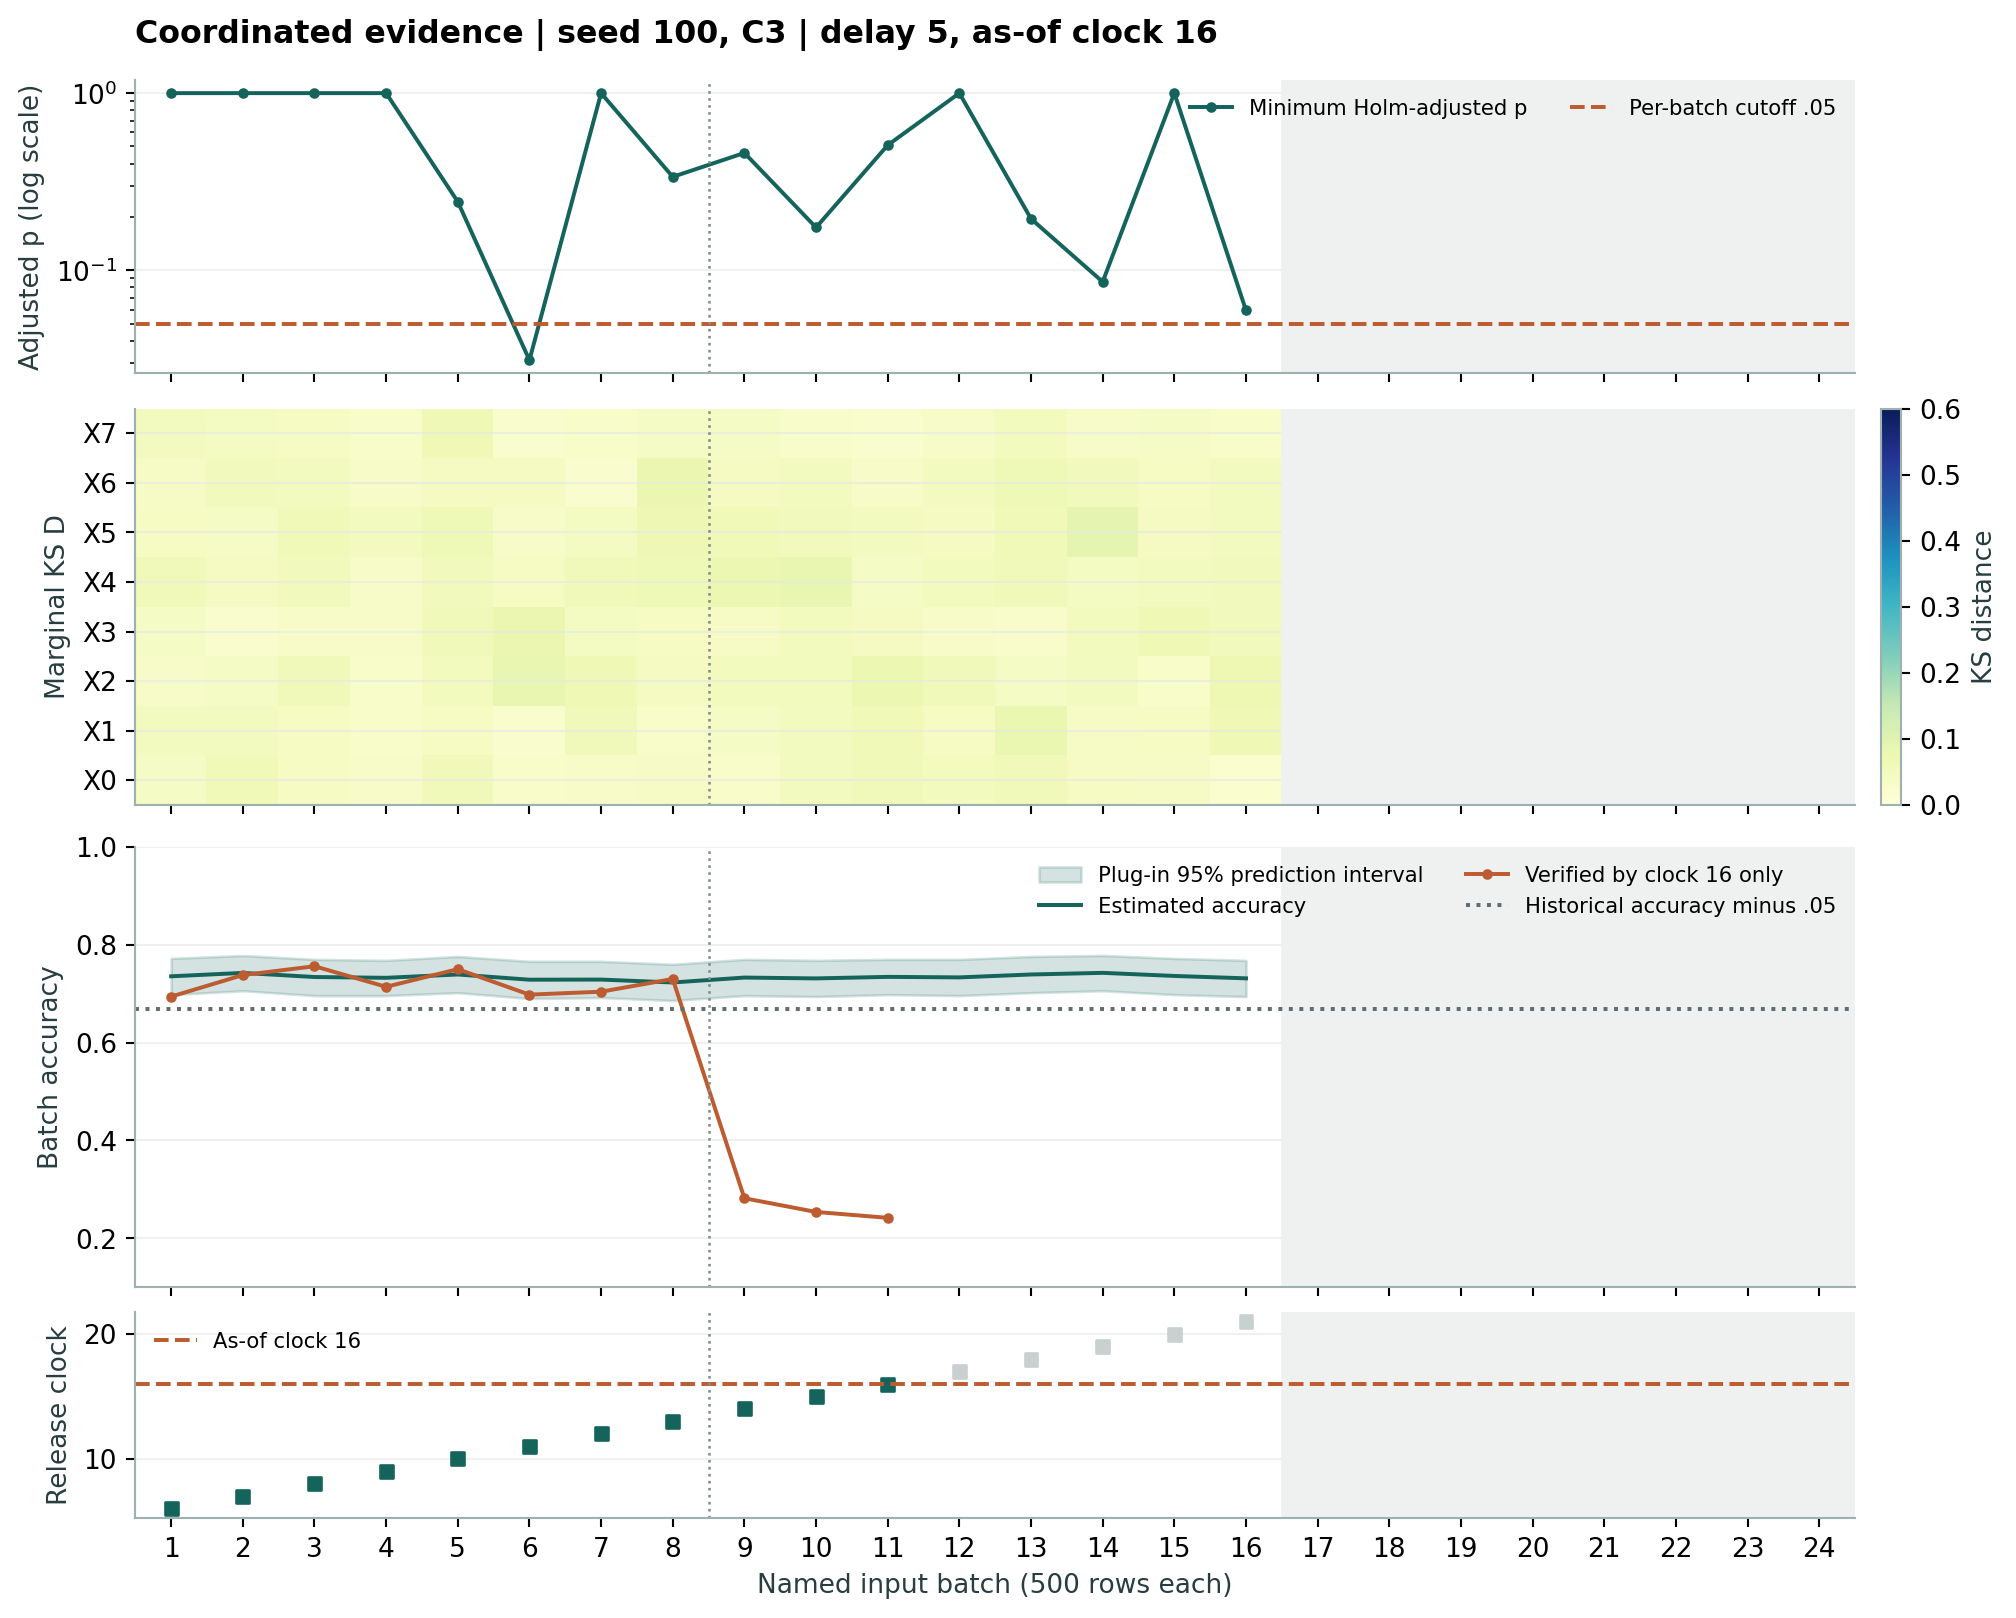
\includegraphics[width=.96\linewidth]{figures/01_coordinated_evidence.png}
\caption{Existing v1 coordinated evidence example (seed 100, C3, delay 5, clock 16). Verified outcomes are available only for released cohorts; future inputs are hidden. Figure is retained from the versioned v1 report.}
\end{figure}

\section{Validation and reproducibility status}
The current source audit confirmed the v1 prediction-before-release order, absence of labels from the feature scoring interface, unit marginal variance in C6, and the adaptation runner's persist-before-release sequence. Evaluation code resamples seed-level summaries rather than treating batches as independent bootstrap units. Current evaluator aggregation and all v2 path invariants have not received a full fresh rerun in this Day 1 session.

Historical validation receipt \texttt{reports/phase3/validation/complete\_package\_validation.json} records 48 passing workspace tests, 8 passing isolated package tests, exact reproducibility comparisons for v1 and adaptation, and package help-command checks. These are historical receipt claims, not newly executed results here. The v1 browser receipt records checks of as-of label boundaries and coordinated panel selection. The current session independently checked SHA-256 for the submitted Phase 2 DOCX, implementation PDF, submitted archive, v1 archives, and research archives; values are in \texttt{HASHES.sha256} and the audit checkpoint.

\begin{sloppypar}
Reproduction commands for a full clean v1 rerun are provided in \path{docs/phase3/23I-2581_23I-2604_Phase3_Reproduction.md}; adaptation commands are in \path{docs/phase3/ADAPTATION_PROTOCOL.md}. The expected interpreter is \path{C:/Users/hp/anaconda3/python.exe}. Exact historical reproduction claims and environment versions are preserved in the validation receipts. The one-session audit did not rerun those expensive pipelines.
\end{sloppypar}

\section{Limitations and deviations}
All core evidence is generated synthetic data. The 30 seeds quantify variability under this generator, not independent real-world replications. Calibration and interval behavior can fail under conditional change; plug-in intervals omit calibration uncertainty. Feature importance is not causal. The concern score is not a calibrated harm probability, and no population-level harm is certified. V2 and adaptation were selected after earlier outcomes and are explicitly outcome-informed extensions. External dataset evaluation, causal discovery, neural adaptation, selective labels, and participant studies remain deferred. No participants or human benefits are claimed.

\section{Preservation and versioning}
\begin{sloppypar}
The submitted Phase 2 DOCX, Phase 3 implementation brief, submitted Phase 3 archive, historical v1 archives, and prior v2/adaptation evidence are preserved. This Day 1 edition is stored under \path{docs/phase3/research_improvement_day1/}; its source and build outputs do not replace any submitted artifact. Hashes should be recomputed before handoff. Tectonic 0.17.0 compiled this report. Page images were rendered and visually inspected; clean package extraction remains pending.
\end{sloppypar}

\bibliographystyle{plain}
\bibliography{REFERENCES}
\end{document}
